\section{Bits}
\frame{\tableofcontents[currentsection]}

\begin{frame}
  \frametitle{Bit Manipulation}
  \begin{itemize}
    \item Instead of using an \texttt{int} as a number\dots
    \item \dots we can use it as an "array" of bits
    \item It is possible to use signed integers
    \item But unsigned integers are easier to work with
  \end{itemize}
\end{frame}

\begin{frame}
  \frametitle{Binary Integer Literal}
  \begin{itemize}
    \item Literal: code representation of a value
    \item Programming languages offer literals for built-in types
  \end{itemize}
  \vskip4mm
  \structure{Examples}
  \begin{center}
    \begin{tabular}{ll}
      \toprule
      \textbf{Type} & \textbf{Example} \\
      \midrule
      String & \texttt{"abc"} \\
      Boolean & \texttt{true} \\
      Integer (decimal) & \texttt{51} \\
      Integer (hexadecimal) & \texttt{0xA12F} \\
      \color{red} Integer (binary) & \color{red}\texttt{0b10010101} \\
      \bottomrule
    \end{tabular}
  \end{center}
\end{frame}

\subsubsection{And}
\frame{\tableofcontents[currentsubsection]}

\begin{frame}
  \frametitle{Logical AND}
  \begin{itemize}
    \item You already know the \texttt{\&\&} operator
    \item It operates on \texttt{bools} and yields a \texttt{bool}
  \end{itemize}
  \begin{center}
    \begin{tabular}{ccc}
      \toprule
      \texttt{a} & \texttt{b} & \texttt{a \&\& b} \\
      \midrule
      \texttt{false} & \texttt{false} & \texttt{false} \\
      \texttt{false} & \texttt{true} & \texttt{false} \\
      \texttt{true} & \texttt{false} & \texttt{false} \\
      \texttt{true} & \texttt{true} & \texttt{true} \\
      \bottomrule
    \end{tabular}
  \end{center}
\end{frame}

\begin{frame}
  \frametitle{Bitwise AND}
  \begin{itemize}
    \item Let's replace \texttt{bool}s by bits
    \item Use \texttt{\&} instead of \texttt{\&\&}
  \end{itemize}
  \begin{center}
    \begin{tabular}{ccc}
      \toprule
      \texttt{a} & \texttt{b} & \texttt{a \& b} \\
      \midrule
      \texttt{0} & \texttt{0} & \texttt{0} \\
      \texttt{0} & \texttt{1} & \texttt{0} \\
      \texttt{1} & \texttt{0} & \texttt{0} \\
      \texttt{1} & \texttt{1} & \texttt{1} \\
      \bottomrule
    \end{tabular}
  \end{center}
\end{frame}

\begin{frame}
  \frametitle{Bitwise AND}
  \begin{itemize}
    \item \texttt{\&} operates on integral types
    \item Apply the AND rule to each bit separately
  \end{itemize}
  \begin{center}
    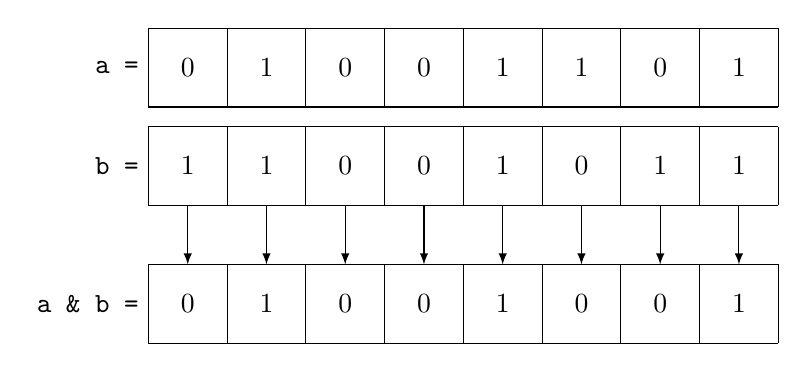
\begin{tikzpicture}
      \draw (0,0) grid (8,1);
      \node[anchor=east,font=\ttfamily] at (0,0.5) {a = };
      \foreach[count=\i,evaluate={\i-0.5} as \x] \v in {0,1,0,0,1,1,0,1} {
        \node at (\x, 0.5) {\v};
      }
      \begin{scope}[yshift=-1.25cm]
        \draw (0,0) grid (8,1);
      \node[anchor=east,font=\ttfamily] at (0,0.5) {b = };
        \foreach[count=\i,evaluate={\i-0.5} as \x] \v in {1,1,0,0,1,0,1,1} {
          \node at (\x, 0.5) {\v};
        }
      \end{scope}

      \begin{scope}[yshift=-1.25cm]
        \foreach[count=\i,evaluate={\i-0.5} as \x] \v in {1,...,8} {
          \draw[-latex] (\x,0) -- ++(0,-0.75);
        }
      \end{scope}

      \begin{scope}[yshift=-3cm]
        \draw (0,0) grid (8,1);
        \node[anchor=east,font=\ttfamily] at (0,0.5) {a \& b = };
        \foreach[count=\i,evaluate={\i-0.5} as \x] \v in {0,1,0,0,1,0,0,1} {
          \node at (\x, 0.5) {\v};
        }
      \end{scope}
    \end{tikzpicture}
  \end{center}
  \vskip2mm
  \begin{center} \ttfamily
    0b01001101 \& 0b11001011 == 0b01001001
  \end{center}
\end{frame}

\subsubsection{Or}
\frame{\tableofcontents[currentsubsection]}

\begin{frame}
  \frametitle{Logical OR}
  \begin{itemize}
    \item You already know the \texttt{||} operator
    \item It operates on \texttt{bools} and yields a \texttt{bool}
  \end{itemize}
  \begin{center}
    \begin{tabular}{ccc}
      \toprule
      \texttt{a} & \texttt{b} & \texttt{a || b} \\
      \midrule
      \texttt{false} & \texttt{false} & \texttt{false} \\
      \texttt{false} & \texttt{true} & \texttt{true} \\
      \texttt{true} & \texttt{false} & \texttt{true} \\
      \texttt{true} & \texttt{true} & \texttt{true} \\
      \bottomrule
    \end{tabular}
  \end{center}
\end{frame}

\begin{frame}
  \frametitle{Bitwise OR}
  \begin{itemize}
    \item Operates on bits instead of \texttt{bool}s
    \item Use \texttt{|} instead of \texttt{||}
  \end{itemize}
  \begin{center}
    \begin{tabular}{ccc}
      \toprule
      \texttt{a} & \texttt{b} & \texttt{a | b} \\
      \midrule
      \texttt{0} & \texttt{0} & \texttt{0} \\
      \texttt{0} & \texttt{1} & \texttt{1} \\
      \texttt{1} & \texttt{0} & \texttt{1} \\
      \texttt{1} & \texttt{1} & \texttt{1} \\
      \bottomrule
    \end{tabular}
  \end{center}
\end{frame}

\begin{frame}
  \frametitle{Bitwise OR}
  \begin{itemize}
    \item \texttt{|} operates on integral types
    \item Apply the OR rule to each bit separately
  \end{itemize}
  \begin{center}
    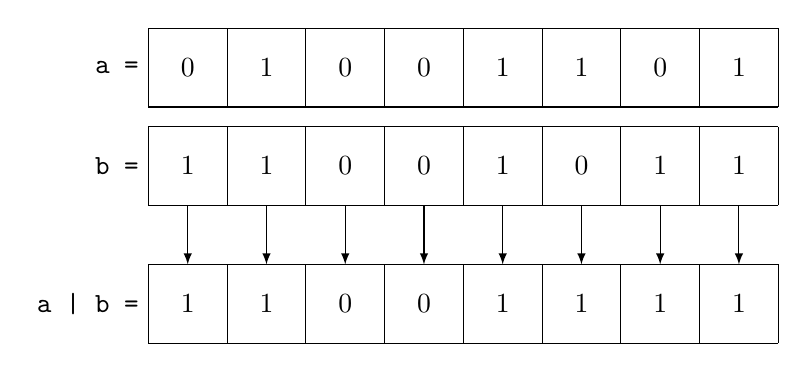
\begin{tikzpicture}
      \draw (0,0) grid (8,1);
      \node[anchor=east,font=\ttfamily] at (0,0.5) {a = };
      \foreach[count=\i,evaluate={\i-0.5} as \x] \v in {0,1,0,0,1,1,0,1} {
        \node at (\x, 0.5) {\v};
      }
      \begin{scope}[yshift=-1.25cm]
        \draw (0,0) grid (8,1);
        \node[anchor=east,font=\ttfamily] at (0,0.5) {b = };
        \foreach[count=\i,evaluate={\i-0.5} as \x] \v in {1,1,0,0,1,0,1,1} {
          \node at (\x, 0.5) {\v};
        }
      \end{scope}

      \begin{scope}[yshift=-1.25cm]
        \foreach[count=\i,evaluate={\i-0.5} as \x] \v in {1,...,8} {
          \draw[-latex] (\x,0) -- ++(0,-0.75);
        }
      \end{scope}

      \begin{scope}[yshift=-3cm]
        \draw (0,0) grid (8,1);
        \node[anchor=east,font=\ttfamily] at (0,0.5) {a | b = };
        \foreach[count=\i,evaluate={\i-0.5} as \x] \v in {1,1,0,0,1,1,1,1} {
          \node at (\x, 0.5) {\v};
        }
      \end{scope}
    \end{tikzpicture}
  \end{center}
  \vskip2mm
  \begin{center} \ttfamily
    0b01001101 | 0b11001011 == 0b11001111
  \end{center}
\end{frame}

\subsubsection{Not}
\frame{\tableofcontents[currentsubsection]}

\begin{frame}
  \frametitle{Logical NOT}
  \begin{itemize}
    \item You already know the \texttt{!} operator
    \item It operates on a single \texttt{bool} and yields a \texttt{bool}
  \end{itemize}
  \begin{center}
    \begin{tabular}{cc}
      \toprule
      \texttt{a} & \texttt{!a} \\
      \midrule
      \texttt{false} & \texttt{true} \\
      \texttt{true} & \texttt{false} \\
      \bottomrule
    \end{tabular}
  \end{center}
\end{frame}

\begin{frame}
  \frametitle{Bitwise NOT}
  \begin{itemize}
    \item Operates on bits instead of \texttt{bool}s
    \item Use \texttt{\NOT} instead of \texttt{!}
  \end{itemize}
  \begin{center}
    \begin{tabular}{ccc}
      \toprule
      \texttt{a} & \texttt{\NOT a} \\
      \midrule
      \texttt{0} & \texttt{1} \\
      \texttt{1} & \texttt{0} \\
      \bottomrule
    \end{tabular}
  \end{center}
\end{frame}

\begin{frame}
  \frametitle{Bitwise NOT}
  \begin{itemize}
    \item \texttt{\NOT} operates on an integral operand
    \item Apply the NOT rule to each bit separately
  \end{itemize}
  \begin{center}
    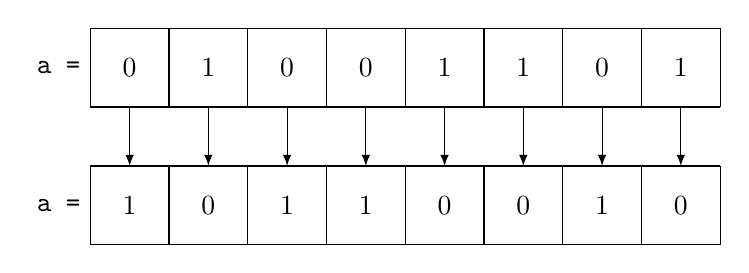
\begin{tikzpicture}
      \draw (0,0) grid (8,1);
      \node[anchor=east,font=\ttfamily] at (0,0.5) {a = };
      \foreach[count=\i,evaluate={\i-0.5} as \x] \v in {0,1,0,0,1,1,0,1} {
        \node at (\x, 0.5) {\v};
      }

      \foreach[count=\i,evaluate={\i-0.5} as \x] \v in {1,...,8} {
        \draw[-latex] (\x,0) -- ++(0,-0.75);
      }

      \begin{scope}[yshift=-1.75cm]
        \draw (0,0) grid (8,1);
        \node[anchor=east,font=\ttfamily] at (0,0.5) {\NOT a = };
        \foreach[count=\i,evaluate={\i-0.5} as \x] \v in {1,0,1,1,0,0,1,0} {
          \node at (\x, 0.5) {\v};
        }
      \end{scope}
    \end{tikzpicture}
  \end{center}
  \vskip2mm
  \begin{center} \ttfamily
    \NOT 0b01001101 == 0b10110010
  \end{center}
\end{frame}

\subsubsection{Xor}
\frame{\tableofcontents[currentsubsection]}

\begin{frame}
  \frametitle{Logical XOR}
  \begin{itemize}
    \item Consider inequality \texttt{a != b} on \texttt{bool}s
    \item Yields \texttt{true} only if \texttt{a} and \texttt{b} are different
    \item Corresponds to XOR (exclusive OR)
  \end{itemize}
  \begin{center}
    \begin{tabular}{ccc}
      \toprule
      \texttt{a} & \texttt{b} & \texttt{a != b} \\
      \midrule
      \texttt{false} & \texttt{false} & \texttt{false} \\
      \texttt{false} & \texttt{true} & \texttt{true} \\
      \texttt{true} & \texttt{false} & \texttt{true} \\
      \texttt{true} & \texttt{true} & \texttt{false} \\
      \bottomrule
    \end{tabular}
  \end{center}
\end{frame}

\begin{frame}
  \frametitle{Bitwise XOR}
  \begin{itemize}
    \item Bitwise exclusive OR is denoted \texttt{a \XOR\ b}
    \item Yields \texttt{1} is bits are unequal, otherwise \texttt{0}
  \end{itemize}
  \begin{center}
    \begin{tabular}{ccc}
      \toprule
      \texttt{a} & \texttt{b} & \texttt{a \XOR b} \\
      \midrule
      \texttt{0} & \texttt{0} & \texttt{0} \\
      \texttt{0} & \texttt{1} & \texttt{1} \\
      \texttt{1} & \texttt{0} & \texttt{1} \\
      \texttt{1} & \texttt{1} & \texttt{0} \\
      \bottomrule
    \end{tabular}
  \end{center}
\end{frame}

\begin{frame}
  \frametitle{Bitwise XOR}
  \begin{center}
    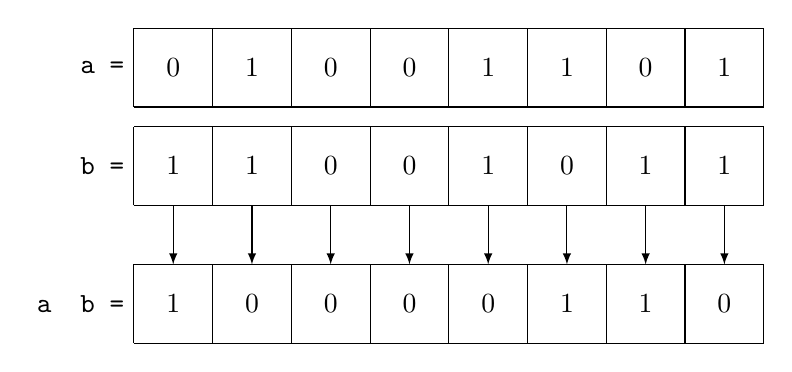
\begin{tikzpicture}
      \draw (0,0) grid (8,1);
      \node[anchor=east,font=\ttfamily] at (0,0.5) {a = };
      \foreach[count=\i,evaluate={\i-0.5} as \x] \v in {0,1,0,0,1,1,0,1} {
        \node at (\x, 0.5) {\v};
      }
      \begin{scope}[yshift=-1.25cm]
        \draw (0,0) grid (8,1);
        \node[anchor=east,font=\ttfamily] at (0,0.5) {b = };
        \foreach[count=\i,evaluate={\i-0.5} as \x] \v in {1,1,0,0,1,0,1,1} {
          \node at (\x, 0.5) {\v};
        }
      \end{scope}

      \begin{scope}[yshift=-1.25cm]
        \foreach[count=\i,evaluate={\i-0.5} as \x] \v in {1,...,8} {
          \draw[-latex] (\x,0) -- ++(0,-0.75);
        }
      \end{scope}

      \begin{scope}[yshift=-3cm]
        \draw (0,0) grid (8,1);
        \node[anchor=east,font=\ttfamily] at (0,0.5) {a \XOR\ b = };
        \foreach[count=\i,evaluate={\i-0.5} as \x] \v in {1,0,0,0,0,1,1,0} {
          \node at (\x, 0.5) {\v};
        }
      \end{scope}
    \end{tikzpicture}
  \end{center}
  \vskip2mm
  \begin{center} \ttfamily
    0b01001101 \XOR\ 0b11001011 == 0b10000110
  \end{center}
\end{frame}

